\documentclass[twoside]{book}

% Packages required by doxygen
\usepackage{fixltx2e}
\usepackage{calc}
\usepackage{doxygen}
\usepackage[export]{adjustbox} % also loads graphicx
\usepackage{graphicx}
\usepackage[utf8]{inputenc}
\usepackage{makeidx}
\usepackage{multicol}
\usepackage{multirow}
\PassOptionsToPackage{warn}{textcomp}
\usepackage{textcomp}
\usepackage[nointegrals]{wasysym}
\usepackage[table]{xcolor}

% Font selection
\usepackage[T1]{fontenc}
\usepackage[scaled=.90]{helvet}
\usepackage{courier}
\usepackage{amssymb}
\usepackage{sectsty}
\renewcommand{\familydefault}{\sfdefault}
\allsectionsfont{%
  \fontseries{bc}\selectfont%
  \color{darkgray}%
}
\renewcommand{\DoxyLabelFont}{%
  \fontseries{bc}\selectfont%
  \color{darkgray}%
}
\newcommand{\+}{\discretionary{\mbox{\scriptsize$\hookleftarrow$}}{}{}}

% Page & text layout
\usepackage{geometry}
\geometry{%
  a4paper,%
  top=2.5cm,%
  bottom=2.5cm,%
  left=2.5cm,%
  right=2.5cm%
}
\tolerance=750
\hfuzz=15pt
\hbadness=750
\setlength{\emergencystretch}{15pt}
\setlength{\parindent}{0cm}
\setlength{\parskip}{3ex plus 2ex minus 2ex}
\makeatletter
\renewcommand{\paragraph}{%
  \@startsection{paragraph}{4}{0ex}{-1.0ex}{1.0ex}{%
    \normalfont\normalsize\bfseries\SS@parafont%
  }%
}
\renewcommand{\subparagraph}{%
  \@startsection{subparagraph}{5}{0ex}{-1.0ex}{1.0ex}{%
    \normalfont\normalsize\bfseries\SS@subparafont%
  }%
}
\makeatother

% Headers & footers
\usepackage{fancyhdr}
\pagestyle{fancyplain}
\fancyhead[LE]{\fancyplain{}{\bfseries\thepage}}
\fancyhead[CE]{\fancyplain{}{}}
\fancyhead[RE]{\fancyplain{}{\bfseries\leftmark}}
\fancyhead[LO]{\fancyplain{}{\bfseries\rightmark}}
\fancyhead[CO]{\fancyplain{}{}}
\fancyhead[RO]{\fancyplain{}{\bfseries\thepage}}
\fancyfoot[LE]{\fancyplain{}{}}
\fancyfoot[CE]{\fancyplain{}{}}
\fancyfoot[RE]{\fancyplain{}{\bfseries\scriptsize Generated by Doxygen }}
\fancyfoot[LO]{\fancyplain{}{\bfseries\scriptsize Generated by Doxygen }}
\fancyfoot[CO]{\fancyplain{}{}}
\fancyfoot[RO]{\fancyplain{}{}}
\renewcommand{\footrulewidth}{0.4pt}
\renewcommand{\chaptermark}[1]{%
  \markboth{#1}{}%
}
\renewcommand{\sectionmark}[1]{%
  \markright{\thesection\ #1}%
}

% Indices & bibliography
\usepackage{natbib}
\usepackage[titles]{tocloft}
\setcounter{tocdepth}{3}
\setcounter{secnumdepth}{5}
\makeindex

% Hyperlinks (required, but should be loaded last)
\usepackage{ifpdf}
\ifpdf
  \usepackage[pdftex,pagebackref=true]{hyperref}
\else
  \usepackage[ps2pdf,pagebackref=true]{hyperref}
\fi
\hypersetup{%
  colorlinks=true,%
  linkcolor=blue,%
  citecolor=blue,%
  unicode%
}

% Custom commands
\newcommand{\clearemptydoublepage}{%
  \newpage{\pagestyle{empty}\cleardoublepage}%
}

\usepackage{caption}
\captionsetup{labelsep=space,justification=centering,font={bf},singlelinecheck=off,skip=4pt,position=top}

%===== C O N T E N T S =====

\begin{document}

% Titlepage & ToC
\hypersetup{pageanchor=false,
             bookmarksnumbered=true,
             pdfencoding=unicode
            }
\pagenumbering{roman}
\begin{titlepage}
\vspace*{7cm}
\begin{center}%
{\Large Q-\/learning for Navigating a 2-\/D grid }\\
\vspace*{1cm}
{\large Generated by Doxygen 1.8.11}\\
\end{center}
\end{titlepage}
\clearemptydoublepage
\tableofcontents
\clearemptydoublepage
\pagenumbering{arabic}
\hypersetup{pageanchor=true}

%--- Begin generated contents ---
\chapter{Class Index}
\section{Class List}
Here are the classes, structs, unions and interfaces with brief descriptions\+:\begin{DoxyCompactList}
\item\contentsline{section}{\hyperlink{classQclass}{Qclass} }{\pageref{classQclass}}{}
\end{DoxyCompactList}

\chapter{File Index}
\section{File List}
Here is a list of all files with brief descriptions\+:\begin{DoxyCompactList}
\item\contentsline{section}{/home/sudartion/workspace/\+Q-\/learning-\/for-\/2\+D-\/\+Occupancy-\/\+Grid/app/\hyperlink{Learn_8cpp}{Learn.\+cpp} \\*\+: Qlearning class member function declarations }{\pageref{Learn_8cpp}}{}
\item\contentsline{section}{/home/sudartion/workspace/\+Q-\/learning-\/for-\/2\+D-\/\+Occupancy-\/\+Grid/app/\hyperlink{app_2main_8cpp}{main.\+cpp} \\*\+: Qlearning class member function declarations }{\pageref{app_2main_8cpp}}{}
\item\contentsline{section}{/home/sudartion/workspace/\+Q-\/learning-\/for-\/2\+D-\/\+Occupancy-\/\+Grid/include/\hyperlink{lib_8hpp}{lib.\+hpp} \\*\+: Qlearning class member function declarations }{\pageref{lib_8hpp}}{}
\item\contentsline{section}{/home/sudartion/workspace/\+Q-\/learning-\/for-\/2\+D-\/\+Occupancy-\/\+Grid/include/\hyperlink{Qlearn-class_8hpp}{Qlearn-\/class.\+hpp} \\*\+: Qlearning class members }{\pageref{Qlearn-class_8hpp}}{}
\item\contentsline{section}{/home/sudartion/workspace/\+Q-\/learning-\/for-\/2\+D-\/\+Occupancy-\/\+Grid/test/\hyperlink{test_2main_8cpp}{main.\+cpp} \\*\+: Test functions for the Q learning class }{\pageref{test_2main_8cpp}}{}
\item\contentsline{section}{/home/sudartion/workspace/\+Q-\/learning-\/for-\/2\+D-\/\+Occupancy-\/\+Grid/test/\hyperlink{test_8cpp}{test.\+cpp} \\*\+: Test functions for the Q learning class }{\pageref{test_8cpp}}{}
\end{DoxyCompactList}

\chapter{Class Documentation}
\hypertarget{classQclass}{}\section{Qclass Class Reference}
\label{classQclass}\index{Qclass@{Qclass}}


{\ttfamily \#include $<$Qlearn-\/class.\+hpp$>$}

\subsection*{Public Member Functions}
\begin{DoxyCompactItemize}
\item 
\hyperlink{classQclass_ab6bd1cc95cf90e0c1759ba26f57bd5a3}{$\sim$\+Qclass} ()
\begin{DoxyCompactList}\small\item\em Destructor for the class. \end{DoxyCompactList}\end{DoxyCompactItemize}
\subsection*{State}
\begin{DoxyCompactItemize}
\item 
int \hyperlink{classQclass_ac7e42ac35f89616a6036aabd29e928f7}{state}
\item 
int \hyperlink{classQclass_ab060f941f076f76056d8276594893b54}{grid} \mbox{[}50\mbox{]}\mbox{[}50\mbox{]} = \{\}
\item 
int \hyperlink{classQclass_a1a72661a0262d34a0b4326c0ef654a1e}{action}
\item 
double \hyperlink{classQclass_a84fb95339b401c66efa8c47d1426c1fe}{Q} \mbox{[}2500\mbox{]}\mbox{[}4\mbox{]} = \{\}
\item 
bool \hyperlink{classQclass_a04ec3a45dc94d48bf13e27c3f18b8399}{restart} = false
\item 
int \hyperlink{classQclass_ab8b70c6206387fcf4dd9ff6d4d7cb2a6}{goal\+\_\+x} = 3
\item 
int \hyperlink{classQclass_a492324bfb266e2ed4f0faf4487fad979}{goal\+\_\+y} = 0
\item 
double \hyperlink{classQclass_addcd4274dbe26c15264572bf354cbd79}{learn\+\_\+rate} = 0.\+5
\item 
double \hyperlink{classQclass_aca70cf943c9d29dcea36f7c6a46d9f0e}{disc\+\_\+rew} = 0.\+8
\item 
void \hyperlink{classQclass_ae9f97c2f18fc7d9e307e35994901da2a}{create\+Grid} ()
\begin{DoxyCompactList}\small\item\em Creates the grid with obstacles in it.\+Obstacle added to .txt file to plot. \end{DoxyCompactList}\item 
int \hyperlink{classQclass_a834429fa9e01f1b283a0caada7802be3}{find\+State} (int x, int y)
\begin{DoxyCompactList}\small\item\em Finds current state based on x,y position. \end{DoxyCompactList}\item 
int \hyperlink{classQclass_a9037e62a852d506051538adfcf7e2337}{det\+Action} (int \hyperlink{classQclass_ac7e42ac35f89616a6036aabd29e928f7}{state})
\begin{DoxyCompactList}\small\item\em Determines the action to be performed next. \end{DoxyCompactList}\item 
int \hyperlink{classQclass_a4155dabacd6e918c6288bd453e956547}{rewardfunc} (int prev\+Action, int x, int y)
\begin{DoxyCompactList}\small\item\em Assigns a reward based on action chosen. \end{DoxyCompactList}\item 
int \hyperlink{classQclass_acf95c3d28bc5ab0409a0824abf36fe04}{futurereward} (int \hyperlink{classQclass_ac7e42ac35f89616a6036aabd29e928f7}{state})
\begin{DoxyCompactList}\small\item\em Finds the highest reward considering future rewards. \end{DoxyCompactList}\item 
void \hyperlink{classQclass_a9feff64b8b2c661a16f4229215957541}{Qupdate} (int prev\+Action, int prev\+State, int x, int y, int \hyperlink{classQclass_ac7e42ac35f89616a6036aabd29e928f7}{state})
\begin{DoxyCompactList}\small\item\em Updates Q table based on action taken for given grid position. \end{DoxyCompactList}\item 
int \hyperlink{classQclass_a4bf8b5d57ca3cf93ee0b9e74c5eeb5f8}{Train} ()
\begin{DoxyCompactList}\small\item\em Performs the training for the Q learning algorithm for a large number of trials. \end{DoxyCompactList}\item 
int \hyperlink{classQclass_a475913f6b4aa9508a501007260afe96b}{execute} ()
\begin{DoxyCompactList}\small\item\em Finds the path from start to goal node using optimized Q table. \end{DoxyCompactList}\item 
int \hyperlink{classQclass_aecebf934f5a3500e2bf2ae98ca02093c}{plot} ()
\begin{DoxyCompactList}\small\item\em Plots the path and obstacles stored in txt files. \end{DoxyCompactList}\end{DoxyCompactItemize}


\subsection{Constructor \& Destructor Documentation}
\index{Qclass@{Qclass}!````~Qclass@{$\sim$\+Qclass}}
\index{````~Qclass@{$\sim$\+Qclass}!Qclass@{Qclass}}
\subsubsection[{\texorpdfstring{$\sim$\+Qclass()}{~Qclass()}}]{\setlength{\rightskip}{0pt plus 5cm}Qclass\+::$\sim$\+Qclass (
\begin{DoxyParamCaption}
{}
\end{DoxyParamCaption}
)}\hypertarget{classQclass_ab6bd1cc95cf90e0c1759ba26f57bd5a3}{}\label{classQclass_ab6bd1cc95cf90e0c1759ba26f57bd5a3}


Destructor for the class. 



\subsection{Member Function Documentation}
\index{Qclass@{Qclass}!create\+Grid@{create\+Grid}}
\index{create\+Grid@{create\+Grid}!Qclass@{Qclass}}
\subsubsection[{\texorpdfstring{create\+Grid()}{createGrid()}}]{\setlength{\rightskip}{0pt plus 5cm}void Qclass\+::create\+Grid (
\begin{DoxyParamCaption}
{}
\end{DoxyParamCaption}
)}\hypertarget{classQclass_ae9f97c2f18fc7d9e307e35994901da2a}{}\label{classQclass_ae9f97c2f18fc7d9e307e35994901da2a}


Creates the grid with obstacles in it.\+Obstacle added to .txt file to plot. 

\index{Qclass@{Qclass}!det\+Action@{det\+Action}}
\index{det\+Action@{det\+Action}!Qclass@{Qclass}}
\subsubsection[{\texorpdfstring{det\+Action(int state)}{detAction(int state)}}]{\setlength{\rightskip}{0pt plus 5cm}int Qclass\+::det\+Action (
\begin{DoxyParamCaption}
\item[{int}]{state}
\end{DoxyParamCaption}
)}\hypertarget{classQclass_a9037e62a852d506051538adfcf7e2337}{}\label{classQclass_a9037e62a852d506051538adfcf7e2337}


Determines the action to be performed next. 


\begin{DoxyParams}{Parameters}
{\em state} & -\/\+Current state of the robot. \\
\hline
\end{DoxyParams}
\begin{DoxyReturn}{Returns}
action decided out of the possible 4 choices (up,down,left and right) 
\end{DoxyReturn}
\index{Qclass@{Qclass}!execute@{execute}}
\index{execute@{execute}!Qclass@{Qclass}}
\subsubsection[{\texorpdfstring{execute()}{execute()}}]{\setlength{\rightskip}{0pt plus 5cm}int Qclass\+::execute (
\begin{DoxyParamCaption}
{}
\end{DoxyParamCaption}
)}\hypertarget{classQclass_a475913f6b4aa9508a501007260afe96b}{}\label{classQclass_a475913f6b4aa9508a501007260afe96b}


Finds the path from start to goal node using optimized Q table. 

\begin{DoxyReturn}{Returns}
0 when goal node is reached 
\end{DoxyReturn}
\index{Qclass@{Qclass}!find\+State@{find\+State}}
\index{find\+State@{find\+State}!Qclass@{Qclass}}
\subsubsection[{\texorpdfstring{find\+State(int x, int y)}{findState(int x, int y)}}]{\setlength{\rightskip}{0pt plus 5cm}int Qclass\+::find\+State (
\begin{DoxyParamCaption}
\item[{int}]{x, }
\item[{int}]{y}
\end{DoxyParamCaption}
)}\hypertarget{classQclass_a834429fa9e01f1b283a0caada7802be3}{}\label{classQclass_a834429fa9e01f1b283a0caada7802be3}


Finds current state based on x,y position. 


\begin{DoxyParams}{Parameters}
{\em x} & grid position x \\
\hline
{\em y} & grid position y \\
\hline
\end{DoxyParams}
\begin{DoxyReturn}{Returns}
state current 
\end{DoxyReturn}
\index{Qclass@{Qclass}!futurereward@{futurereward}}
\index{futurereward@{futurereward}!Qclass@{Qclass}}
\subsubsection[{\texorpdfstring{futurereward(int state)}{futurereward(int state)}}]{\setlength{\rightskip}{0pt plus 5cm}int Qclass\+::futurereward (
\begin{DoxyParamCaption}
\item[{int}]{new\+\_\+state}
\end{DoxyParamCaption}
)}\hypertarget{classQclass_acf95c3d28bc5ab0409a0824abf36fe04}{}\label{classQclass_acf95c3d28bc5ab0409a0824abf36fe04}


Finds the highest reward considering future rewards. 


\begin{DoxyParams}{Parameters}
{\em new\+\_\+state} & is the next state of the robot for action taken in current state \\
\hline
\end{DoxyParams}
\begin{DoxyReturn}{Returns}
curr\+Max table value for the state 
\end{DoxyReturn}
\index{Qclass@{Qclass}!plot@{plot}}
\index{plot@{plot}!Qclass@{Qclass}}
\subsubsection[{\texorpdfstring{plot()}{plot()}}]{\setlength{\rightskip}{0pt plus 5cm}int Qclass\+::plot (
\begin{DoxyParamCaption}
{}
\end{DoxyParamCaption}
)}\hypertarget{classQclass_aecebf934f5a3500e2bf2ae98ca02093c}{}\label{classQclass_aecebf934f5a3500e2bf2ae98ca02093c}


Plots the path and obstacles stored in txt files. 

\begin{DoxyReturn}{Returns}
0 when path plotting is complete 
\end{DoxyReturn}
\index{Qclass@{Qclass}!Qupdate@{Qupdate}}
\index{Qupdate@{Qupdate}!Qclass@{Qclass}}
\subsubsection[{\texorpdfstring{Qupdate(int prev\+Action, int prev\+State, int x, int y, int state)}{Qupdate(int prevAction, int prevState, int x, int y, int state)}}]{\setlength{\rightskip}{0pt plus 5cm}void Qclass\+::\+Qupdate (
\begin{DoxyParamCaption}
\item[{int}]{last\+Action, }
\item[{int}]{last\+State, }
\item[{int}]{x, }
\item[{int}]{y, }
\item[{int}]{new\+\_\+state}
\end{DoxyParamCaption}
)}\hypertarget{classQclass_a9feff64b8b2c661a16f4229215957541}{}\label{classQclass_a9feff64b8b2c661a16f4229215957541}


Updates Q table based on action taken for given grid position. 


\begin{DoxyParams}{Parameters}
{\em last\+State} & \\
\hline
{\em last\+Action} & \\
\hline
{\em x} & \\
\hline
{\em y} & \\
\hline
{\em new\+\_\+state} & \\
\hline
\end{DoxyParams}
\index{Qclass@{Qclass}!rewardfunc@{rewardfunc}}
\index{rewardfunc@{rewardfunc}!Qclass@{Qclass}}
\subsubsection[{\texorpdfstring{rewardfunc(int prev\+Action, int x, int y)}{rewardfunc(int prevAction, int x, int y)}}]{\setlength{\rightskip}{0pt plus 5cm}int Qclass\+::rewardfunc (
\begin{DoxyParamCaption}
\item[{int}]{last\+Action, }
\item[{int}]{x, }
\item[{int}]{y}
\end{DoxyParamCaption}
)}\hypertarget{classQclass_a4155dabacd6e918c6288bd453e956547}{}\label{classQclass_a4155dabacd6e918c6288bd453e956547}


Assigns a reward based on action chosen. 


\begin{DoxyParams}{Parameters}
{\em last\+Action} & \\
\hline
{\em x} & \\
\hline
{\em y} & \\
\hline
\end{DoxyParams}
\begin{DoxyReturn}{Returns}
reward assigned 
\end{DoxyReturn}
\index{Qclass@{Qclass}!Train@{Train}}
\index{Train@{Train}!Qclass@{Qclass}}
\subsubsection[{\texorpdfstring{Train()}{Train()}}]{\setlength{\rightskip}{0pt plus 5cm}int Qclass\+::\+Train (
\begin{DoxyParamCaption}
{}
\end{DoxyParamCaption}
)}\hypertarget{classQclass_a4bf8b5d57ca3cf93ee0b9e74c5eeb5f8}{}\label{classQclass_a4bf8b5d57ca3cf93ee0b9e74c5eeb5f8}


Performs the training for the Q learning algorithm for a large number of trials. 

\begin{DoxyReturn}{Returns}
0 when training is complete 
\end{DoxyReturn}


\subsection{Member Data Documentation}
\index{Qclass@{Qclass}!action@{action}}
\index{action@{action}!Qclass@{Qclass}}
\subsubsection[{\texorpdfstring{action}{action}}]{\setlength{\rightskip}{0pt plus 5cm}int Qclass\+::action}\hypertarget{classQclass_a1a72661a0262d34a0b4326c0ef654a1e}{}\label{classQclass_a1a72661a0262d34a0b4326c0ef654a1e}
\index{Qclass@{Qclass}!disc\+\_\+rew@{disc\+\_\+rew}}
\index{disc\+\_\+rew@{disc\+\_\+rew}!Qclass@{Qclass}}
\subsubsection[{\texorpdfstring{disc\+\_\+rew}{disc_rew}}]{\setlength{\rightskip}{0pt plus 5cm}double Qclass\+::disc\+\_\+rew = 0.\+8}\hypertarget{classQclass_aca70cf943c9d29dcea36f7c6a46d9f0e}{}\label{classQclass_aca70cf943c9d29dcea36f7c6a46d9f0e}
\index{Qclass@{Qclass}!goal\+\_\+x@{goal\+\_\+x}}
\index{goal\+\_\+x@{goal\+\_\+x}!Qclass@{Qclass}}
\subsubsection[{\texorpdfstring{goal\+\_\+x}{goal_x}}]{\setlength{\rightskip}{0pt plus 5cm}int Qclass\+::goal\+\_\+x = 3}\hypertarget{classQclass_ab8b70c6206387fcf4dd9ff6d4d7cb2a6}{}\label{classQclass_ab8b70c6206387fcf4dd9ff6d4d7cb2a6}
\index{Qclass@{Qclass}!goal\+\_\+y@{goal\+\_\+y}}
\index{goal\+\_\+y@{goal\+\_\+y}!Qclass@{Qclass}}
\subsubsection[{\texorpdfstring{goal\+\_\+y}{goal_y}}]{\setlength{\rightskip}{0pt plus 5cm}int Qclass\+::goal\+\_\+y = 0}\hypertarget{classQclass_a492324bfb266e2ed4f0faf4487fad979}{}\label{classQclass_a492324bfb266e2ed4f0faf4487fad979}
\index{Qclass@{Qclass}!grid@{grid}}
\index{grid@{grid}!Qclass@{Qclass}}
\subsubsection[{\texorpdfstring{grid}{grid}}]{\setlength{\rightskip}{0pt plus 5cm}int Qclass\+::grid\mbox{[}50\mbox{]}\mbox{[}50\mbox{]} = \{\}}\hypertarget{classQclass_ab060f941f076f76056d8276594893b54}{}\label{classQclass_ab060f941f076f76056d8276594893b54}
\index{Qclass@{Qclass}!learn\+\_\+rate@{learn\+\_\+rate}}
\index{learn\+\_\+rate@{learn\+\_\+rate}!Qclass@{Qclass}}
\subsubsection[{\texorpdfstring{learn\+\_\+rate}{learn_rate}}]{\setlength{\rightskip}{0pt plus 5cm}double Qclass\+::learn\+\_\+rate = 0.\+5}\hypertarget{classQclass_addcd4274dbe26c15264572bf354cbd79}{}\label{classQclass_addcd4274dbe26c15264572bf354cbd79}
\index{Qclass@{Qclass}!Q@{Q}}
\index{Q@{Q}!Qclass@{Qclass}}
\subsubsection[{\texorpdfstring{Q}{Q}}]{\setlength{\rightskip}{0pt plus 5cm}double Qclass\+::Q\mbox{[}2500\mbox{]}\mbox{[}4\mbox{]} = \{\}}\hypertarget{classQclass_a84fb95339b401c66efa8c47d1426c1fe}{}\label{classQclass_a84fb95339b401c66efa8c47d1426c1fe}
\index{Qclass@{Qclass}!restart@{restart}}
\index{restart@{restart}!Qclass@{Qclass}}
\subsubsection[{\texorpdfstring{restart}{restart}}]{\setlength{\rightskip}{0pt plus 5cm}bool Qclass\+::restart = false}\hypertarget{classQclass_a04ec3a45dc94d48bf13e27c3f18b8399}{}\label{classQclass_a04ec3a45dc94d48bf13e27c3f18b8399}
\index{Qclass@{Qclass}!state@{state}}
\index{state@{state}!Qclass@{Qclass}}
\subsubsection[{\texorpdfstring{state}{state}}]{\setlength{\rightskip}{0pt plus 5cm}Qclass\+::state}\hypertarget{classQclass_ac7e42ac35f89616a6036aabd29e928f7}{}\label{classQclass_ac7e42ac35f89616a6036aabd29e928f7}


The documentation for this class was generated from the following files\+:\begin{DoxyCompactItemize}
\item 
/home/sudartion/workspace/\+Q-\/learning-\/for-\/2\+D-\/\+Occupancy-\/\+Grid/include/\hyperlink{Qlearn-class_8hpp}{Qlearn-\/class.\+hpp}\item 
/home/sudartion/workspace/\+Q-\/learning-\/for-\/2\+D-\/\+Occupancy-\/\+Grid/app/\hyperlink{Learn_8cpp}{Learn.\+cpp}\end{DoxyCompactItemize}

\chapter{File Documentation}
\hypertarget{app_2CMakeLists_8txt}{}\section{/home/sudartion/workspace/\+Q-\/learning-\/for-\/2\+D-\/\+Occupancy-\/\+Grid/app/\+C\+Make\+Lists.txt File Reference}
\label{app_2CMakeLists_8txt}\index{/home/sudartion/workspace/\+Q-\/learning-\/for-\/2\+D-\/\+Occupancy-\/\+Grid/app/\+C\+Make\+Lists.\+txt@{/home/sudartion/workspace/\+Q-\/learning-\/for-\/2\+D-\/\+Occupancy-\/\+Grid/app/\+C\+Make\+Lists.\+txt}}
\subsection*{Functions}
\begin{DoxyCompactItemize}
\item 
\hyperlink{app_2CMakeLists_8txt_a6b1182e92df972472c51304e784b2e37}{add\+\_\+executable} (shell-\/app main.\+cpp) include\+\_\+directories(\$
\end{DoxyCompactItemize}


\subsection{Function Documentation}
\index{app/\+C\+Make\+Lists.\+txt@{app/\+C\+Make\+Lists.\+txt}!add\+\_\+executable@{add\+\_\+executable}}
\index{add\+\_\+executable@{add\+\_\+executable}!app/\+C\+Make\+Lists.\+txt@{app/\+C\+Make\+Lists.\+txt}}
\subsubsection[{\texorpdfstring{add\+\_\+executable(shell-\/app main.\+cpp) include\+\_\+directories(\$}{add_executable(shell-app main.cpp) include_directories($}}]{\setlength{\rightskip}{0pt plus 5cm}add\+\_\+executable (
\begin{DoxyParamCaption}
\item[{shell-\/app main.}]{cpp}
\end{DoxyParamCaption}
)}\hypertarget{app_2CMakeLists_8txt_a6b1182e92df972472c51304e784b2e37}{}\label{app_2CMakeLists_8txt_a6b1182e92df972472c51304e784b2e37}

\hypertarget{test_2CMakeLists_8txt}{}\section{/home/sudartion/workspace/\+Q-\/learning-\/for-\/2\+D-\/\+Occupancy-\/\+Grid/test/\+C\+Make\+Lists.txt File Reference}
\label{test_2CMakeLists_8txt}\index{/home/sudartion/workspace/\+Q-\/learning-\/for-\/2\+D-\/\+Occupancy-\/\+Grid/test/\+C\+Make\+Lists.\+txt@{/home/sudartion/workspace/\+Q-\/learning-\/for-\/2\+D-\/\+Occupancy-\/\+Grid/test/\+C\+Make\+Lists.\+txt}}
\subsection*{Functions}
\begin{DoxyCompactItemize}
\item 
\hyperlink{test_2CMakeLists_8txt_af8680b0c55887bf90463d8bb729e26e2}{set} (G\+T\+E\+S\+T\+\_\+\+S\+H\+U\+F\+F\+LE 1) \hyperlink{app_2CMakeLists_8txt_a6b1182e92df972472c51304e784b2e37}{add\+\_\+executable}(cpp-\/test main.\+cpp test.\+cpp../app/Learn.\+cpp) target\+\_\+include\+\_\+directories(cpp-\/test P\+U\+B\+L\+I\+C../vendor/googletest/googletest/include \$
\end{DoxyCompactItemize}


\subsection{Function Documentation}
\index{test/\+C\+Make\+Lists.\+txt@{test/\+C\+Make\+Lists.\+txt}!set@{set}}
\index{set@{set}!test/\+C\+Make\+Lists.\+txt@{test/\+C\+Make\+Lists.\+txt}}
\subsubsection[{\texorpdfstring{set(\+G\+T\+E\+S\+T\+\_\+\+S\+H\+U\+F\+F\+L\+E 1) add\+\_\+executable(cpp-\/test main.\+cpp test.\+cpp../app/\+Learn.\+cpp) target\+\_\+include\+\_\+directories(cpp-\/test P\+U\+B\+L\+I\+C../vendor/googletest/googletest/include \$}{set(GTEST_SHUFFLE 1) add_executable(cpp-test main.cpp test.cpp../app/Learn.cpp) target_include_directories(cpp-test PUBLIC../vendor/googletest/googletest/include $}}]{\setlength{\rightskip}{0pt plus 5cm}set (
\begin{DoxyParamCaption}
\item[{G\+T\+E\+S\+T\+\_\+\+S\+H\+U\+F\+F\+LE}]{1}
\end{DoxyParamCaption}
)}\hypertarget{test_2CMakeLists_8txt_af8680b0c55887bf90463d8bb729e26e2}{}\label{test_2CMakeLists_8txt_af8680b0c55887bf90463d8bb729e26e2}

\hypertarget{Learn_8cpp}{}\section{/home/sudartion/workspace/\+Q-\/learning-\/for-\/2\+D-\/\+Occupancy-\/\+Grid/app/\+Learn.cpp File Reference}
\label{Learn_8cpp}\index{/home/sudartion/workspace/\+Q-\/learning-\/for-\/2\+D-\/\+Occupancy-\/\+Grid/app/\+Learn.\+cpp@{/home/sudartion/workspace/\+Q-\/learning-\/for-\/2\+D-\/\+Occupancy-\/\+Grid/app/\+Learn.\+cpp}}


\+: Qlearning class member function declarations  


{\ttfamily \#include $<$stdlib.\+h$>$}\\*
{\ttfamily \#include $<$iostream$>$}\\*
{\ttfamily \#include $<$fstream$>$}\\*
{\ttfamily \#include \char`\"{}Qlearn-\/class.\+hpp\char`\"{}}\\*
{\ttfamily \#include \char`\"{}../gnuplot-\/cpp/gnuplot\+\_\+i.\+hpp\char`\"{}}\\*
Include dependency graph for Learn.\+cpp\+:
\nopagebreak
\begin{figure}[H]
\begin{center}
\leavevmode
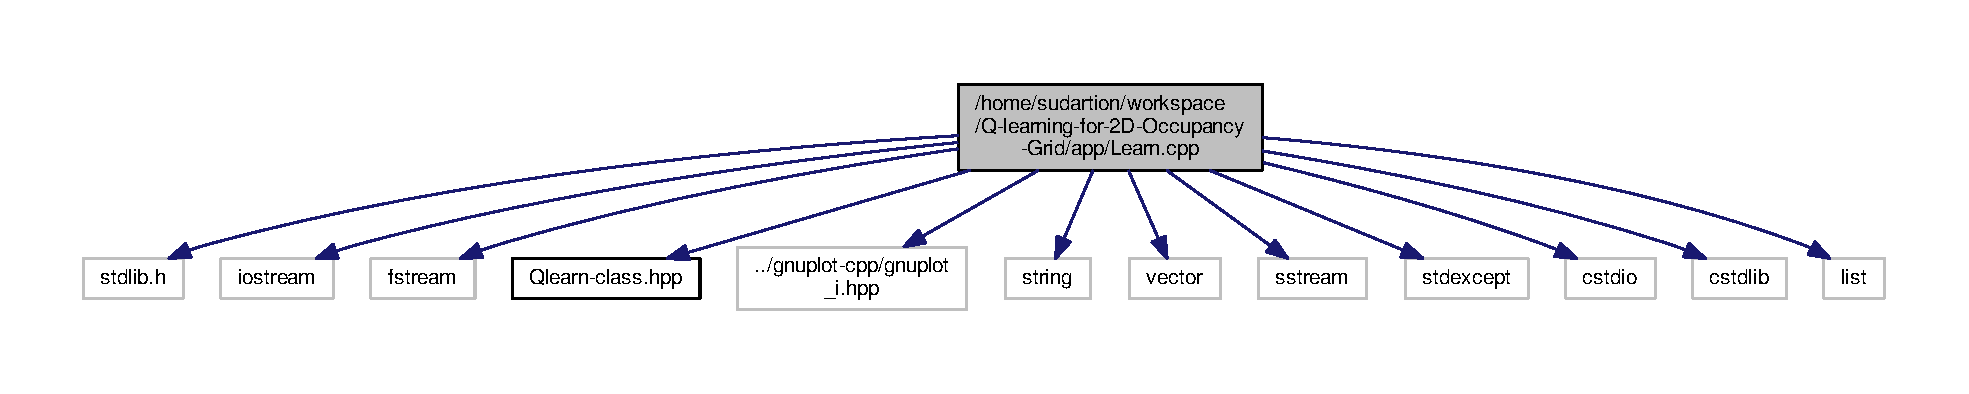
\includegraphics[width=350pt]{Learn_8cpp__incl}
\end{center}
\end{figure}
This graph shows which files directly or indirectly include this file\+:
\nopagebreak
\begin{figure}[H]
\begin{center}
\leavevmode
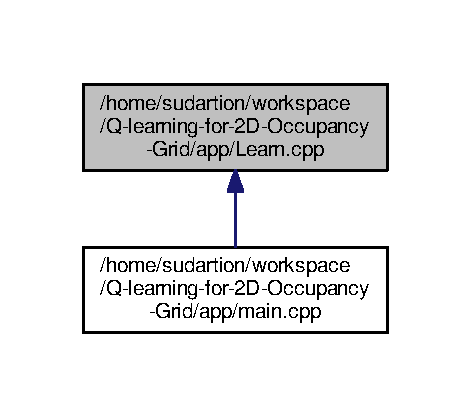
\includegraphics[width=226pt]{Learn_8cpp__dep__incl}
\end{center}
\end{figure}


\subsection{Detailed Description}
\+: Qlearning class member function declarations 

\begin{DoxyAuthor}{Author}
\+: Sudarshan Raghunathan 
\end{DoxyAuthor}
\begin{DoxyCopyright}{Copyright}
\+: 2017 Sudarshan Raghunathan 
\end{DoxyCopyright}

\hypertarget{app_2main_8cpp}{}\section{/home/sudartion/workspace/\+Q-\/learning-\/for-\/2\+D-\/\+Occupancy-\/\+Grid/app/main.cpp File Reference}
\label{app_2main_8cpp}\index{/home/sudartion/workspace/\+Q-\/learning-\/for-\/2\+D-\/\+Occupancy-\/\+Grid/app/main.\+cpp@{/home/sudartion/workspace/\+Q-\/learning-\/for-\/2\+D-\/\+Occupancy-\/\+Grid/app/main.\+cpp}}


\+: Qlearning class member function declarations  


{\ttfamily \#include $<$lib.\+hpp$>$}\\*
{\ttfamily \#include $<$iostream$>$}\\*
{\ttfamily \#include \char`\"{}Qlearn-\/class.\+hpp\char`\"{}}\\*
{\ttfamily \#include \char`\"{}Learn.\+cpp\char`\"{}}\\*
Include dependency graph for main.\+cpp\+:
\nopagebreak
\begin{figure}[H]
\begin{center}
\leavevmode
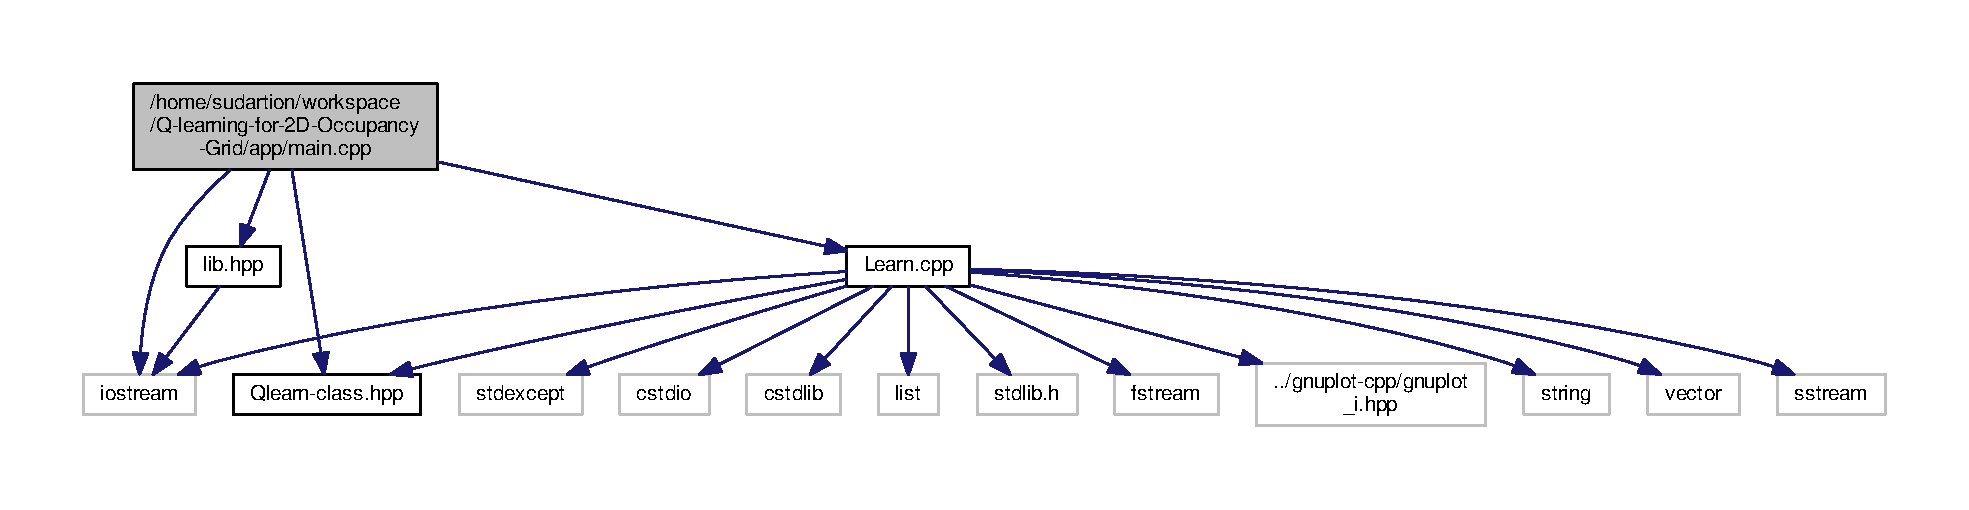
\includegraphics[width=350pt]{app_2main_8cpp__incl}
\end{center}
\end{figure}
\subsection*{Functions}
\begin{DoxyCompactItemize}
\item 
int \hyperlink{app_2main_8cpp_ae66f6b31b5ad750f1fe042a706a4e3d4}{main} ()
\begin{DoxyCompactList}\small\item\em Main function to execute the code. \end{DoxyCompactList}\end{DoxyCompactItemize}


\subsection{Detailed Description}
\+: Qlearning class member function declarations 

\begin{DoxyAuthor}{Author}
\+: Sudarshan Raghunathan 
\end{DoxyAuthor}
\begin{DoxyCopyright}{Copyright}
\+: 2017 Sudarshan Raghunathan 
\end{DoxyCopyright}


\subsection{Function Documentation}
\index{app/main.\+cpp@{app/main.\+cpp}!main@{main}}
\index{main@{main}!app/main.\+cpp@{app/main.\+cpp}}
\subsubsection[{\texorpdfstring{main()}{main()}}]{\setlength{\rightskip}{0pt plus 5cm}int main (
\begin{DoxyParamCaption}
{}
\end{DoxyParamCaption}
)}\hypertarget{app_2main_8cpp_ae66f6b31b5ad750f1fe042a706a4e3d4}{}\label{app_2main_8cpp_ae66f6b31b5ad750f1fe042a706a4e3d4}


Main function to execute the code. 


\hypertarget{test_2main_8cpp}{}\section{/home/sudartion/workspace/\+Q-\/learning-\/for-\/2\+D-\/\+Occupancy-\/\+Grid/test/main.cpp File Reference}
\label{test_2main_8cpp}\index{/home/sudartion/workspace/\+Q-\/learning-\/for-\/2\+D-\/\+Occupancy-\/\+Grid/test/main.\+cpp@{/home/sudartion/workspace/\+Q-\/learning-\/for-\/2\+D-\/\+Occupancy-\/\+Grid/test/main.\+cpp}}


\+: Test functions for the Q learning class  


{\ttfamily \#include $<$gtest/gtest.\+h$>$}\\*
Include dependency graph for main.\+cpp\+:
\nopagebreak
\begin{figure}[H]
\begin{center}
\leavevmode
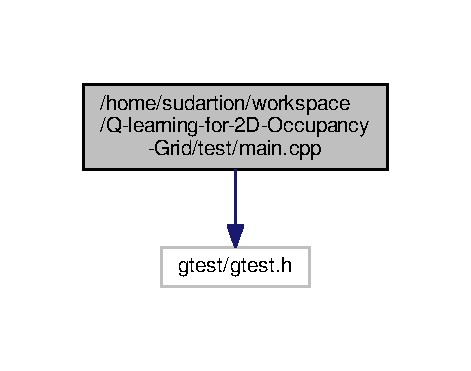
\includegraphics[width=226pt]{test_2main_8cpp__incl}
\end{center}
\end{figure}
\subsection*{Functions}
\begin{DoxyCompactItemize}
\item 
int \hyperlink{test_2main_8cpp_a3c04138a5bfe5d72780bb7e82a18e627}{main} (int argc, char $\ast$$\ast$argv)
\begin{DoxyCompactList}\small\item\em Main function to run tests. \end{DoxyCompactList}\end{DoxyCompactItemize}


\subsection{Detailed Description}
\+: Test functions for the Q learning class 

\begin{DoxyAuthor}{Author}
\+: Sudarshan Raghunathan 
\end{DoxyAuthor}
\begin{DoxyCopyright}{Copyright}
\+: 2017 Sudarshan Raghunathan 
\end{DoxyCopyright}


\subsection{Function Documentation}
\index{test/main.\+cpp@{test/main.\+cpp}!main@{main}}
\index{main@{main}!test/main.\+cpp@{test/main.\+cpp}}
\subsubsection[{\texorpdfstring{main(int argc, char $\ast$$\ast$argv)}{main(int argc, char **argv)}}]{\setlength{\rightskip}{0pt plus 5cm}int main (
\begin{DoxyParamCaption}
\item[{int}]{argc, }
\item[{char $\ast$$\ast$}]{argv}
\end{DoxyParamCaption}
)}\hypertarget{test_2main_8cpp_a3c04138a5bfe5d72780bb7e82a18e627}{}\label{test_2main_8cpp_a3c04138a5bfe5d72780bb7e82a18e627}


Main function to run tests. 


\begin{DoxyParams}{Parameters}
{\em argc} & \\
\hline
{\em argv} & \\
\hline
\end{DoxyParams}

\hypertarget{lib_8hpp}{}\section{/home/sudartion/workspace/\+Q-\/learning-\/for-\/2\+D-\/\+Occupancy-\/\+Grid/include/lib.hpp File Reference}
\label{lib_8hpp}\index{/home/sudartion/workspace/\+Q-\/learning-\/for-\/2\+D-\/\+Occupancy-\/\+Grid/include/lib.\+hpp@{/home/sudartion/workspace/\+Q-\/learning-\/for-\/2\+D-\/\+Occupancy-\/\+Grid/include/lib.\+hpp}}


\+: Qlearning class member function declarations  


{\ttfamily \#include $<$iostream$>$}\\*
Include dependency graph for lib.\+hpp\+:
\nopagebreak
\begin{figure}[H]
\begin{center}
\leavevmode
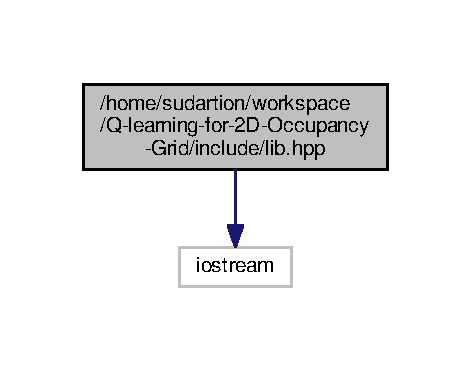
\includegraphics[width=226pt]{lib_8hpp__incl}
\end{center}
\end{figure}
This graph shows which files directly or indirectly include this file\+:
\nopagebreak
\begin{figure}[H]
\begin{center}
\leavevmode
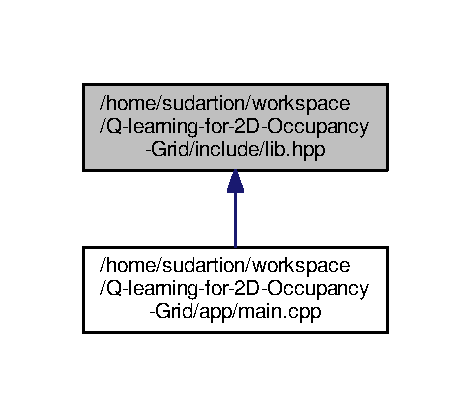
\includegraphics[width=226pt]{lib_8hpp__dep__incl}
\end{center}
\end{figure}
\subsection*{Functions}
\begin{DoxyCompactItemize}
\item 
void \hyperlink{lib_8hpp_a100d09f9a57d44745299c28c63c98745}{dummy} ()
\end{DoxyCompactItemize}


\subsection{Detailed Description}
\+: Qlearning class member function declarations 

\begin{DoxyAuthor}{Author}
\+: Sudarshan Raghunathan 
\end{DoxyAuthor}
\begin{DoxyCopyright}{Copyright}
\+: 2017 Sudarshan Raghunathan 
\end{DoxyCopyright}


\subsection{Function Documentation}
\index{lib.\+hpp@{lib.\+hpp}!dummy@{dummy}}
\index{dummy@{dummy}!lib.\+hpp@{lib.\+hpp}}
\subsubsection[{\texorpdfstring{dummy()}{dummy()}}]{\setlength{\rightskip}{0pt plus 5cm}void dummy (
\begin{DoxyParamCaption}
{}
\end{DoxyParamCaption}
)}\hypertarget{lib_8hpp_a100d09f9a57d44745299c28c63c98745}{}\label{lib_8hpp_a100d09f9a57d44745299c28c63c98745}

\hypertarget{Qlearn-class_8hpp}{}\section{/home/sudartion/workspace/\+Q-\/learning-\/for-\/2\+D-\/\+Occupancy-\/\+Grid/include/\+Qlearn-\/class.hpp File Reference}
\label{Qlearn-class_8hpp}\index{/home/sudartion/workspace/\+Q-\/learning-\/for-\/2\+D-\/\+Occupancy-\/\+Grid/include/\+Qlearn-\/class.\+hpp@{/home/sudartion/workspace/\+Q-\/learning-\/for-\/2\+D-\/\+Occupancy-\/\+Grid/include/\+Qlearn-\/class.\+hpp}}


\+: Qlearning class members  


This graph shows which files directly or indirectly include this file\+:
\nopagebreak
\begin{figure}[H]
\begin{center}
\leavevmode
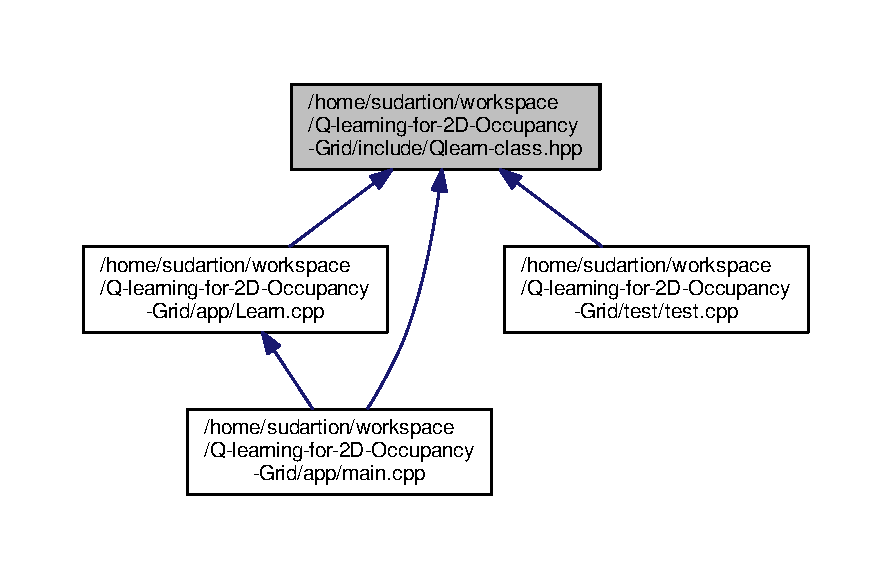
\includegraphics[width=350pt]{Qlearn-class_8hpp__dep__incl}
\end{center}
\end{figure}
\subsection*{Classes}
\begin{DoxyCompactItemize}
\item 
class \hyperlink{classQclass}{Qclass}
\end{DoxyCompactItemize}


\subsection{Detailed Description}
\+: Qlearning class members 

\begin{DoxyAuthor}{Author}
\+: Sudarshan Raghunathan 
\end{DoxyAuthor}
\begin{DoxyCopyright}{Copyright}
\+: 2017 Sudarshan Raghunathan 
\end{DoxyCopyright}

\hypertarget{test_8cpp}{}\section{/home/sudartion/workspace/\+Q-\/learning-\/for-\/2\+D-\/\+Occupancy-\/\+Grid/test/test.cpp File Reference}
\label{test_8cpp}\index{/home/sudartion/workspace/\+Q-\/learning-\/for-\/2\+D-\/\+Occupancy-\/\+Grid/test/test.\+cpp@{/home/sudartion/workspace/\+Q-\/learning-\/for-\/2\+D-\/\+Occupancy-\/\+Grid/test/test.\+cpp}}


\+: Test functions for the Q learning class  


{\ttfamily \#include $<$gtest/gtest.\+h$>$}\\*
{\ttfamily \#include $<$memory$>$}\\*
{\ttfamily \#include $<$fstream$>$}\\*
{\ttfamily \#include \char`\"{}../include/\+Qlearn-\/class.\+hpp\char`\"{}}\\*
Include dependency graph for test.\+cpp\+:
\nopagebreak
\begin{figure}[H]
\begin{center}
\leavevmode
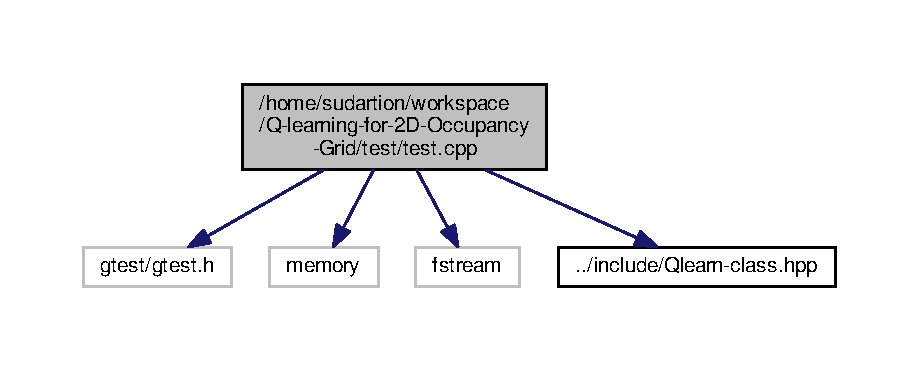
\includegraphics[width=350pt]{test_8cpp__incl}
\end{center}
\end{figure}
\subsection*{Functions}
\begin{DoxyCompactItemize}
\item 
\hyperlink{test_8cpp_a241bcd81e39ef3fa1c2c47d8b6efa6f1}{T\+E\+ST} (\hyperlink{classQclass}{Qclass}, find\+State)
\begin{DoxyCompactList}\small\item\em Helps identify right state for x,y locations. \end{DoxyCompactList}\item 
\hyperlink{test_8cpp_a561c23d473313de5621a2569f68b3e7a}{T\+E\+ST} (\hyperlink{classQclass}{Qclass}, det\+Action)
\begin{DoxyCompactList}\small\item\em Checks if action chosen is between 0 and 3. \end{DoxyCompactList}\item 
\hyperlink{test_8cpp_aad9452b52a85973fe250d2e9d90f6565}{T\+E\+ST} (\hyperlink{classQclass}{Qclass}, rewardfunc)
\begin{DoxyCompactList}\small\item\em Checks if reward is assigned correctly. \end{DoxyCompactList}\item 
\hyperlink{test_8cpp_a3e39acafdfb01f2bef1bd17232ec8ac1}{T\+E\+ST} (\hyperlink{classQclass}{Qclass}, futurereward)
\begin{DoxyCompactList}\small\item\em Helps identify right state for x,y locations. \end{DoxyCompactList}\item 
\hyperlink{test_8cpp_a375bcfbcfcf54810593015b95b37988f}{T\+E\+ST} (\hyperlink{classQclass}{Qclass}, Qupdate)
\begin{DoxyCompactList}\small\item\em Helps identify right state for x,y locations. \end{DoxyCompactList}\item 
\hyperlink{test_8cpp_a8b29e3cdcfd29c1718a8eb41ef9ac4c3}{T\+E\+ST} (\hyperlink{classQclass}{Qclass}, Train)
\begin{DoxyCompactList}\small\item\em Checks if training is completed. \end{DoxyCompactList}\item 
\hyperlink{test_8cpp_adc6592bfeb0f0acb502a92de5b607f27}{T\+E\+ST} (\hyperlink{classQclass}{Qclass}, execute)
\begin{DoxyCompactList}\small\item\em Checks if goal was reached. \end{DoxyCompactList}\item 
\hyperlink{test_8cpp_a99d5559a3a9c7d47f27088ef8baff52b}{T\+E\+ST} (\hyperlink{classQclass}{Qclass}, plot)
\begin{DoxyCompactList}\small\item\em Checks if plot was completed. \end{DoxyCompactList}\item 
\hyperlink{test_8cpp_a370b1d58b6b11ffc7829f8c3a60086d8}{T\+E\+ST} (\hyperlink{classQclass}{Qclass}, noplot)
\begin{DoxyCompactList}\small\item\em Checks output for plotting empty text file. \end{DoxyCompactList}\end{DoxyCompactItemize}


\subsection{Detailed Description}
\+: Test functions for the Q learning class 

\begin{DoxyAuthor}{Author}
\+: Sudarshan Raghunathan 
\end{DoxyAuthor}
\begin{DoxyCopyright}{Copyright}
\+: 2017 Sudarshan Raghunathan 
\end{DoxyCopyright}


\subsection{Function Documentation}
\index{test.\+cpp@{test.\+cpp}!T\+E\+ST@{T\+E\+ST}}
\index{T\+E\+ST@{T\+E\+ST}!test.\+cpp@{test.\+cpp}}
\subsubsection[{\texorpdfstring{T\+E\+S\+T(\+Qclass, find\+State)}{TEST(Qclass, findState)}}]{\setlength{\rightskip}{0pt plus 5cm}T\+E\+ST (
\begin{DoxyParamCaption}
\item[{{\bf Qclass}}]{, }
\item[{find\+State}]{}
\end{DoxyParamCaption}
)}\hypertarget{test_8cpp_a241bcd81e39ef3fa1c2c47d8b6efa6f1}{}\label{test_8cpp_a241bcd81e39ef3fa1c2c47d8b6efa6f1}


Helps identify right state for x,y locations. 

\index{test.\+cpp@{test.\+cpp}!T\+E\+ST@{T\+E\+ST}}
\index{T\+E\+ST@{T\+E\+ST}!test.\+cpp@{test.\+cpp}}
\subsubsection[{\texorpdfstring{T\+E\+S\+T(\+Qclass, det\+Action)}{TEST(Qclass, detAction)}}]{\setlength{\rightskip}{0pt plus 5cm}T\+E\+ST (
\begin{DoxyParamCaption}
\item[{{\bf Qclass}}]{, }
\item[{det\+Action}]{}
\end{DoxyParamCaption}
)}\hypertarget{test_8cpp_a561c23d473313de5621a2569f68b3e7a}{}\label{test_8cpp_a561c23d473313de5621a2569f68b3e7a}


Checks if action chosen is between 0 and 3. 

\index{test.\+cpp@{test.\+cpp}!T\+E\+ST@{T\+E\+ST}}
\index{T\+E\+ST@{T\+E\+ST}!test.\+cpp@{test.\+cpp}}
\subsubsection[{\texorpdfstring{T\+E\+S\+T(\+Qclass, rewardfunc)}{TEST(Qclass, rewardfunc)}}]{\setlength{\rightskip}{0pt plus 5cm}T\+E\+ST (
\begin{DoxyParamCaption}
\item[{{\bf Qclass}}]{, }
\item[{rewardfunc}]{}
\end{DoxyParamCaption}
)}\hypertarget{test_8cpp_aad9452b52a85973fe250d2e9d90f6565}{}\label{test_8cpp_aad9452b52a85973fe250d2e9d90f6565}


Checks if reward is assigned correctly. 

\index{test.\+cpp@{test.\+cpp}!T\+E\+ST@{T\+E\+ST}}
\index{T\+E\+ST@{T\+E\+ST}!test.\+cpp@{test.\+cpp}}
\subsubsection[{\texorpdfstring{T\+E\+S\+T(\+Qclass, futurereward)}{TEST(Qclass, futurereward)}}]{\setlength{\rightskip}{0pt plus 5cm}T\+E\+ST (
\begin{DoxyParamCaption}
\item[{{\bf Qclass}}]{, }
\item[{futurereward}]{}
\end{DoxyParamCaption}
)}\hypertarget{test_8cpp_a3e39acafdfb01f2bef1bd17232ec8ac1}{}\label{test_8cpp_a3e39acafdfb01f2bef1bd17232ec8ac1}


Helps identify right state for x,y locations. 

\index{test.\+cpp@{test.\+cpp}!T\+E\+ST@{T\+E\+ST}}
\index{T\+E\+ST@{T\+E\+ST}!test.\+cpp@{test.\+cpp}}
\subsubsection[{\texorpdfstring{T\+E\+S\+T(\+Qclass, Qupdate)}{TEST(Qclass, Qupdate)}}]{\setlength{\rightskip}{0pt plus 5cm}T\+E\+ST (
\begin{DoxyParamCaption}
\item[{{\bf Qclass}}]{, }
\item[{Qupdate}]{}
\end{DoxyParamCaption}
)}\hypertarget{test_8cpp_a375bcfbcfcf54810593015b95b37988f}{}\label{test_8cpp_a375bcfbcfcf54810593015b95b37988f}


Helps identify right state for x,y locations. 

\index{test.\+cpp@{test.\+cpp}!T\+E\+ST@{T\+E\+ST}}
\index{T\+E\+ST@{T\+E\+ST}!test.\+cpp@{test.\+cpp}}
\subsubsection[{\texorpdfstring{T\+E\+S\+T(\+Qclass, Train)}{TEST(Qclass, Train)}}]{\setlength{\rightskip}{0pt plus 5cm}T\+E\+ST (
\begin{DoxyParamCaption}
\item[{{\bf Qclass}}]{, }
\item[{Train}]{}
\end{DoxyParamCaption}
)}\hypertarget{test_8cpp_a8b29e3cdcfd29c1718a8eb41ef9ac4c3}{}\label{test_8cpp_a8b29e3cdcfd29c1718a8eb41ef9ac4c3}


Checks if training is completed. 

\index{test.\+cpp@{test.\+cpp}!T\+E\+ST@{T\+E\+ST}}
\index{T\+E\+ST@{T\+E\+ST}!test.\+cpp@{test.\+cpp}}
\subsubsection[{\texorpdfstring{T\+E\+S\+T(\+Qclass, execute)}{TEST(Qclass, execute)}}]{\setlength{\rightskip}{0pt plus 5cm}T\+E\+ST (
\begin{DoxyParamCaption}
\item[{{\bf Qclass}}]{, }
\item[{execute}]{}
\end{DoxyParamCaption}
)}\hypertarget{test_8cpp_adc6592bfeb0f0acb502a92de5b607f27}{}\label{test_8cpp_adc6592bfeb0f0acb502a92de5b607f27}


Checks if goal was reached. 

\index{test.\+cpp@{test.\+cpp}!T\+E\+ST@{T\+E\+ST}}
\index{T\+E\+ST@{T\+E\+ST}!test.\+cpp@{test.\+cpp}}
\subsubsection[{\texorpdfstring{T\+E\+S\+T(\+Qclass, plot)}{TEST(Qclass, plot)}}]{\setlength{\rightskip}{0pt plus 5cm}T\+E\+ST (
\begin{DoxyParamCaption}
\item[{{\bf Qclass}}]{, }
\item[{plot}]{}
\end{DoxyParamCaption}
)}\hypertarget{test_8cpp_a99d5559a3a9c7d47f27088ef8baff52b}{}\label{test_8cpp_a99d5559a3a9c7d47f27088ef8baff52b}


Checks if plot was completed. 

\index{test.\+cpp@{test.\+cpp}!T\+E\+ST@{T\+E\+ST}}
\index{T\+E\+ST@{T\+E\+ST}!test.\+cpp@{test.\+cpp}}
\subsubsection[{\texorpdfstring{T\+E\+S\+T(\+Qclass, noplot)}{TEST(Qclass, noplot)}}]{\setlength{\rightskip}{0pt plus 5cm}T\+E\+ST (
\begin{DoxyParamCaption}
\item[{{\bf Qclass}}]{, }
\item[{noplot}]{}
\end{DoxyParamCaption}
)}\hypertarget{test_8cpp_a370b1d58b6b11ffc7829f8c3a60086d8}{}\label{test_8cpp_a370b1d58b6b11ffc7829f8c3a60086d8}


Checks output for plotting empty text file. 


%--- End generated contents ---

% Index
\backmatter
\newpage
\phantomsection
\clearemptydoublepage
\addcontentsline{toc}{chapter}{Index}
\printindex

\end{document}
